\question 以太网帧的最小长度是( )字节
\par\twoch{32}{\textcolor{red}{64}}{128}{256}
\begin{solution}以太网有最小帧长度限制,设置最小帧长是为了区分开噪声和因发生碰撞而异常终止的短帧,它必须要大于64B。
\end{solution}
\question 以太网的数据帧封装如图3-2所示,包含的TCP段中的数据部分最长应该是( ~)

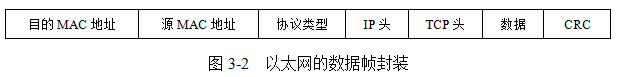
\includegraphics[width=3.33333in,height=0.40625in]{computerassets/25d66fd7ecf9a4aa73d66c4295ed68fb.png}
\par\twoch{1434}{\textcolor{red}{1460}}{1480}{1500}
\begin{solution}以太网帧数据域最大长度为1500B,而IP头和TCP头字段最小长度为20B。因此,用户数据最长为(1500-20-20)B=1460B。
\end{solution}
\question 一个通过以太网传送的IP分组有60B长,其中包括所有头部。若没有使用LLC,则以太网帧中需要(
)填充字节
\par\twoch{4字节}{1440字节}{\textcolor{red}{0字节}}{64字节}
\begin{solution}以太网最小帧的长度是64B,其中包括了在以太网帧头部的地址、类型域、帧尾部的校验和域。这些部分的总共长度是18B,那么加上MAC帧的数据部分60B(整个IP数据报就是MAC帧的数据部分),整个帧长度就为78B,达到了以太网帧最小帧长度64B的要求,所以不需要再添加填充字节。
\end{solution}
